\documentclass[12pt]{article}

\usepackage{amsmath}
\usepackage{amssymb}
\usepackage{enumitem}
\usepackage{geometry}
\geometry{margin=1in}
\usepackage{tikz}
\usetikzlibrary{arrows.meta,decorations.pathmorphing,angles,quotes,calc}

\setlist[enumerate,1]{label=\arabic*.}
\setlist[enumerate,2]{label=\Alph*)}

\begin{document}

\begin{center}
{\Large \textbf{Ultra-Hard Physics Paper}}\\[4pt]
Single Correct Type
\end{center}

\begin{enumerate}

%------------------------------------------------
\item
A small block of mass $m$ carrying charge $q$ is placed on a smooth wedge of mass $M$ which rests on a frictionless horizontal surface. The incline makes an angle $\theta$ with the horizontal. A uniform horizontal electric field $E$ acts toward the right, and the block is released from rest from a point such that its initial vertical height above the base is $h$.

During the subsequent motion, the wedge is free to recoil and no slipping occurs between block and wedge. Consider the combined effects of work done by electric field, constraint relations, and conservation laws to determine the horizontal velocity of the wedge at the instant the block just reaches the bottom edge.

% Q1 Diagram
% Corrected Diagram for Q1
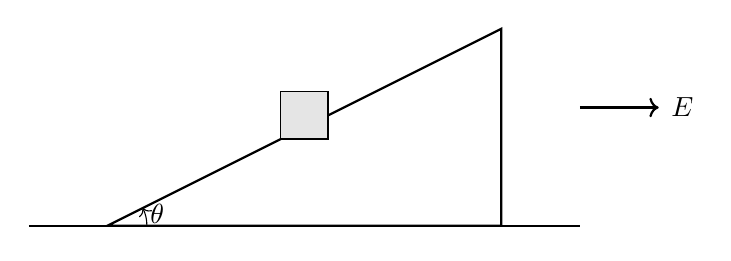
\begin{tikzpicture}[scale=1]
\draw[thick] (-1,0)--(6,0); % ground
\coordinate (A) at (0,0);
\coordinate (B) at (5,0);
\coordinate (C) at (5,2.5);
\draw[thick] (A)--(C)--(B)--cycle;

\draw[fill=gray!20] (2.2,1.1) rectangle (2.8,1.7);

\draw[->,thick] (6,1.5)--(7,1.5);
\node at (7.3,1.5) {$E$};

\pic[draw,->,"$\theta$",angle eccentricity=1.3]
{angle = B--A--C};
\end{tikzpicture}

% Fully Corrected Options for Q1
\begin{enumerate}
\item $\dfrac{m}{M+m}\sqrt{2gh+\dfrac{2qEh\cos\theta}{m\sin\theta}}$
\item $\dfrac{m}{M+m}\sqrt{2gh-\dfrac{2qEh\cos\theta}{m\sin\theta}}$
\item $\sqrt{\dfrac{2mgh}{M+m}}$
\item $\dfrac{m}{M}\sqrt{2gh+\dfrac{2qEh\cos\theta}{m\sin\theta}}$
\end{enumerate}

%------------------------------------------------
\item
A particle of mass $m$ carrying charge $q$ is attached to a light inextensible string of length $l$ fixed at a point. From the lowest point, it is projected horizontally with speed $v$. A uniform vertical electric field $E$ acts upward throughout the motion.

Assuming the motion remains planar and the string remains taut until a certain critical point, determine the minimum initial speed required such that the string just becomes slack at some point during the motion. Carefully account for varying effective gravity and radial force balance at the limiting point.
% Corrected Options for Q2
\begin{enumerate}
\item $\sqrt{5gl-\dfrac{5qEl}{m}}$
\item $\sqrt{3gl-\dfrac{3qEl}{m}}$
\item $\sqrt{2gl-\dfrac{2qEl}{m}}$
\item $\sqrt{gl-\dfrac{qEl}{m}}$
\end{enumerate}



%------------------------------------------------
\item
A conducting rod of length $L$ is placed on two parallel conducting rails forming a closed circuit of total resistance $R$. The entire arrangement is kept fixed in a region where the magnetic field varies with time as $B(t)=B_0(1+\alpha t)$ directed perpendicular to the plane of the circuit.

Neglect self-inductance and assume the rod remains mechanically constrained so that no motional emf arises. Determine the total charge that flows through the circuit between time $t=0$ and $t=T$.

% Q3 Diagram
\begin{tikzpicture}[scale=1]
\draw (0,0)--(5,0);
\draw (0,-1)--(5,-1);
\draw[thick] (2,0)--(2,-1);
\draw[->] (3.5,0.5)--(3.5,1.5);
\node at (3.5,1.8) {$B(t)$};
\node at (2.3,-0.5) {$L$};
\end{tikzpicture}

% Corrected Options for Q3
\begin{enumerate}
\item $\dfrac{B_0L^2\alpha T}{R}$
\item $\dfrac{B_0L^2\alpha T^2}{2R}$
\item $\dfrac{B_0L^2}{R}$
\item zero
\end{enumerate}

%------------------------------------------------
\item
A uniform conducting rod of mass $m$ and length $L$ is pivoted at one end and allowed to execute small angular oscillations about its equilibrium position in a vertical plane. A uniform magnetic field $B$ perpendicular to the plane is suddenly switched on, and the rod has total electrical resistance $R$.

Taking into account electromagnetic damping due to induced currents along the rod and working in the small angle approximation, determine how the natural angular frequency of oscillation is modified to first order in magnetic field strength.

% Q4 Diagram
\begin{tikzpicture}[scale=1]
\draw[fill=black] (0,0) circle (0.05);
\draw[thick] (0,0)--(3,1.5);
\draw[->] (2.5,2)--(2.5,3);
\node at (2.5,3.3) {$B$};
\node at (1.7,1) {$L$};
\end{tikzpicture}

% Corrected Options for Q4
\begin{enumerate}
\item $\sqrt{\dfrac{3g}{2L}}$
\item $\sqrt{\dfrac{3g}{2L}-\dfrac{3B^4L^4}{16m^2R^2}}$
\item $\sqrt{\dfrac{3g}{L}}$
\item $\sqrt{\dfrac{g}{L}}$
\end{enumerate}

%------------------------------------------------
\item
An ideal gas is enclosed in a vertical cylinder of cross-sectional area $A$ by a frictionless piston of mass $M$. The piston is also attached to a vertical spring of force constant $k$. At equilibrium the gas pressure and volume are $P_0$ and $V_0$.

If the piston is displaced slightly and released, the system performs small adiabatic oscillations. Taking into account both restoring forces due to spring and gas compressibility, determine the effective angular frequency of oscillation.

% Q5 Diagram
\begin{tikzpicture}[scale=1]
\draw (0,0)--(3,0)--(3,4)--(0,4);
\draw[fill=gray!20] (0,2)--(3,2);
\draw[thick] (1.5,2)--(1.5,3.5);
\draw[decorate,decoration={coil,aspect=0.3,segment length=3mm}] (1.5,3.5)--(1.5,4);
\node at (1.7,3) {$M$};
\node at (2.6,1) {Gas};
\end{tikzpicture}

\begin{enumerate}
\item $\sqrt{\dfrac{k}{M}}$
\item $\sqrt{\dfrac{k+\gamma P_0A^2/V_0}{M}}$
\item $\sqrt{\dfrac{\gamma P_0A^2}{MV_0}}$
\item $\sqrt{\dfrac{k+\gamma P_0A^2}{M}}$
\end{enumerate}

%------------------------------------------------
\item
A particle of mass $m$ moves under the influence of a central potential
\[
U(r)=-\frac{k}{r}+\frac{\alpha}{r^2}, \quad \alpha>0
\]
and executes a stable circular orbit of radius $r_0$.

Considering small radial perturbations about this orbit, derive the frequency of small radial oscillations by expanding the effective potential about equilibrium and carefully evaluating the curvature term.

\begin{enumerate}
\item $\sqrt{\dfrac{k}{mr_0^3}}$
\item $\sqrt{\dfrac{k}{mr_0^3}-\dfrac{3\alpha}{mr_0^4}}$
\item $\sqrt{\dfrac{k}{mr_0^3}+\dfrac{3\alpha}{mr_0^4}}$
\item $\sqrt{\dfrac{2k}{mr_0^3}}$
\end{enumerate}

%------------------------------------------------
\item
A projectile of mass $m$ carrying charge $q$ is fired from the ground with speed $u$ at an angle $\theta$ above the horizontal in a region where a uniform electric field $E$ acts vertically downward.

Ignoring air resistance and assuming constant field everywhere, determine the horizontal range of the projectile by accounting for the modified effective acceleration and the altered time of flight.

\begin{enumerate}
\item $\dfrac{u^2\sin2\theta}{g+\dfrac{qE}{m}}$
\item $\dfrac{u^2\sin2\theta}{g-\dfrac{qE}{m}}$
\item $\dfrac{u^2\sin2\theta}{g}$
\item $\dfrac{u^2\sin2\theta}{\sqrt{g^2+(qE/m)^2}}$
\end{enumerate}

%------------------------------------------------
\item
Two identical blocks of mass $m$ connected by a light spring of force constant $k$ lie on a frictionless horizontal surface. Block A is given an initial velocity $v$ toward block B. During the compression phase, a constant external force $F$ acts only on block A in the direction of motion.

Determine the maximum compression of the spring using an appropriate non-inertial frame or energy approach while accounting for work done by external force during deformation.

% Corrected Q8 Diagram
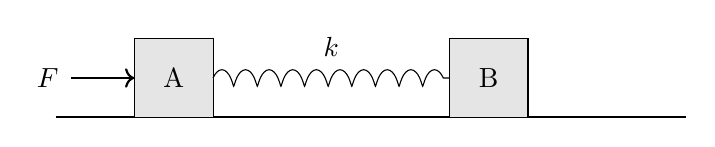
\begin{tikzpicture}[scale=1]

% Ground line
\draw[thick] (-1,0)--(7,0);

% Block A
\draw[fill=gray!20] (0,0)--(1,0)--(1,1)--(0,1)--cycle;
\node at (0.5,0.5) {A};

% Block B
\draw[fill=gray!20] (4,0)--(5,0)--(5,1)--(4,1)--cycle;
\node at (4.5,0.5) {B};

% Spring
\draw[decorate,decoration={coil,aspect=0.35,segment length=3mm,amplitude=3pt}]
(1,0.5)--(4,0.5);

\node at (2.5,0.9) {$k$};

% External force on A (to the right)
\draw[->,thick] (-0.8,0.5)--(0,0.5);
\node at (-1.1,0.5) {$F$};

\end{tikzpicture}

% Fully Correct Options for Q8
\begin{enumerate}
\item $\dfrac{F + \sqrt{F^2 + \tfrac{1}{2}kmv^2}}{k}$
\item $\dfrac{F - \sqrt{F^2 + \tfrac{1}{2}kmv^2}}{k}$
\item $\sqrt{\dfrac{mv^2}{2k}}$
\item $\dfrac{\sqrt{F^2 + kmv^2}}{k}$
\end{enumerate}

%------------------------------------------------
\item
A satellite of mass $m$ moves in a circular orbit of radius $R$ around Earth with orbital speed $v$. It receives a small radial impulse $\Delta v$ directed outward without changing tangential speed instantaneously.

Determine the fractional change in total mechanical energy of the satellite to first order in $\Delta v/v$, carefully expanding the energy expression and considering the perturbative limit.

% Corrected Options for Q9
\begin{enumerate}
\item $2\dfrac{\Delta v}{v}$
\item $\dfrac{\Delta v}{v}$
\item zero
\item $\left(\dfrac{\Delta v}{v}\right)^2$
\end{enumerate}
%------------------------------------------------
\item
A capacitor of capacitance $C$ initially charged to potential $V$ is connected in series with an inductor $L$ and resistor $R$. After the circuit is closed, damped oscillations occur and eventually all currents cease.

Determine the total heat generated in the resistor during the entire transient process by considering conservation of energy in the RLC circuit.

\begin{enumerate}
\item $\dfrac{1}{2}CV^2$
\item $CV^2$
\item $\dfrac{1}{4}CV^2$
\item zero
\end{enumerate}

%------------------------------------------------
\item
A particle moves in a one-dimensional potential
\[
U(x)=\alpha x^4-\beta x^2
\]
which has a double-well structure. The particle is given total mechanical energy equal to the barrier height separating the wells.

Analyze the nature of motion near the unstable equilibrium and determine how the time period behaves as the particle approaches the separatrix trajectory.

\begin{enumerate}
\item finite
\item proportional to amplitude
\item diverges
\item independent of $\alpha$
\end{enumerate}

%------------------------------------------------
\item
A conducting rod of length $L$ rotates with initial angular speed $\omega_0$ about one end in a uniform magnetic field $B$ perpendicular to the plane of rotation. Due to induced currents and resistive losses, the angular speed decreases as
\[
\omega=\omega_0 e^{-\lambda t}.
\]

Determine the total charge that flows through the external resistance during the entire motion by integrating the instantaneous induced emf over time.

% Q12 Diagram
\begin{tikzpicture}[scale=1]
\draw[fill=black] (0,0) circle (0.05);
\draw[thick] (0,0)--(3,0);
\draw[->] (1.5,0.5) arc (20:120:1);
\node at (1.6,1.2) {$\omega$};
\draw[->] (3.5,0.5)--(3.5,1.5);
\node at (3.5,1.8) {$B$};
\node at (1.5,-0.3) {$L$};
\end{tikzpicture}

\begin{enumerate}
\item $\dfrac{BL^2\omega_0}{2R\lambda}$
\item $\dfrac{BL^2\omega_0}{R\lambda}$
\item $\dfrac{BL\omega_0}{R\lambda}$
\item zero
\end{enumerate}

%------------------------------------------------
\item
Two capacitors of capacitances $C$ and $2C$ are individually charged to potential $V$. They are then connected in parallel but with opposite polarity such that charge redistribution occurs.

Determine the final electrostatic energy stored in the system after equilibrium is reached, accounting for charge conservation and potential equalization.

\begin{enumerate}
\item $\dfrac{1}{6}CV^2$
\item $\dfrac{1}{3}CV^2$
\item $\dfrac{1}{2}CV^2$
\item zero
\end{enumerate}

%------------------------------------------------
\item
In the Bohr model of hydrogen atom, an electron is initially in a circular orbit of radius $R$ with angular momentum $L$. Suppose the angular momentum suddenly doubles due to an external perturbation without changing Coulomb interaction form.

Determine the new orbital radius in terms of the original radius by using quantization conditions and centripetal force balance.

\begin{enumerate}
\item $2R$
\item $4R$
\item $R/2$
\item $R/4$
\end{enumerate}

%------------------------------------------------
\item
A particle oscillates in a one-dimensional potential
\[
U(x)=\alpha x^4
\]
with total energy corresponding to maximum displacement $A$.

Determine how the period of oscillation depends on amplitude by performing dimensional analysis or evaluating the integral for time period using energy methods.

\begin{enumerate}
\item constant
\item proportional to $A$
\item proportional to $\dfrac{1}{A}$
\item proportional to $A^2$
\end{enumerate}

%------------------------------------------------

\end{enumerate}

\end{document}